\chapter{Опис додатку з використанням кросс-платформених рішень}
\label{ch2}

\section{Структура проекту в React Native}
\label{section.2.1}

\begin{lstlisting}[style=light, language=Python,label={lst:rn_app_structure},caption=React Native App Layout]
├── App.js (1)
├── Readme.md
├── __tests__ (2)
│ └── App.js
├── android (3)
│ ├── app
│ ├── build
│ ├── build.gradle
│ ├── gradle
│ ├── gradle.properties
│ ├── gradlew
│ ├── gradlew.bat
│ ├── local.properties
│ └── settings.gradle
├── app.json (5)
├── babel.config.js (6)
├── index.js (7)
├── ios (4)
│ ├── BreedRN
│ ├── BreedRN.xcodeproj
│ ├── BreedRN.xcworkspace
│ ├── Podfile
│ ├── Podfile.lock
│ └── Pods
├── metro.config.js (8)
├── node_modules (11)
├── package-lock.json (10)
└── package.json (9)
\end{lstlisting}

\begin{enumerate}
    \item \textbf{App.js} сирцевий код нашого додатку
    \item \textbf{\_\_tests\_\_} сирцевий код тестів
    \item \textbf{android} сирцевий код платформеного коду Android
    \item \textbf{ios} сирцевий код платформеного коду iOS
    \item \textbf{app.json} конфігурує багато речей, від назви вашого додатка до піктограми до заставки, і навіть схеми глибоких зв’язків та ключів API для використання для деяких служб
    \item \textbf{babel.config.js} конфігурує Babel - це набір інструментів, який в основному використовується для перетворення коду ECMAScript 2015+ у зворотну сумісну версію JavaScript у поточних та старих браузерах або середовищах.
    \item \textbf{index.js} точка входу для React Native з цього файлу Javascript Engine вивантажує в пам'ять логіку додатку
    \item \textbf{metro.config.js} конфігурує Metro пакувальник JavaScript для платформ Android та iOS
    \item \textbf{package.json} конфігурує дерево залежностей або бібліотек, що використовує проект
    \item \textbf{package-lock.json} файл що описує повністю дерево залежностей, таким чином створює відтворюване середовище
    \item \textbf{node\_modules} репозиторій артефактів або сирцевого коду всіх Javascript пакетів, що використовує проект
\end{enumerate}

\section{Архітектура додатку React Native}
\label{section.2.2}
В реалізації додатку React Native ми використали систему звротніх викликів або так званих "хуків".
Наприклад, \textbf{useState} - це Хук, що дозволяє додавати стан React до функціональних компонентів.

"useState" оголошує "змінну стану" та повертає пару значень: поточний стан та функцію, яка його оновлює.
Наша змінна називається, data ми можемо називати її як завгодно, наприклад banana \ref{lst:rn_state_hooks}.

Використовуючи useEffect хук, ми повідомляємо React, що наш компонент повинен виконати додаткову фунцію після рендерингу.
React запам'ятає передану нами функцію (яку ми будемо називати "ефектом") і викличе її пізніше після оновлення UI нашого додатку.

Ефект котрий ми створили буде виконаний при ініціалізації додатку. І як результат виконання ми отримаємо дані з локальної бази які ми і відобразимо (див. на \ref{fig:rn_realm})).

\begin{figure}
    \begin{center}
        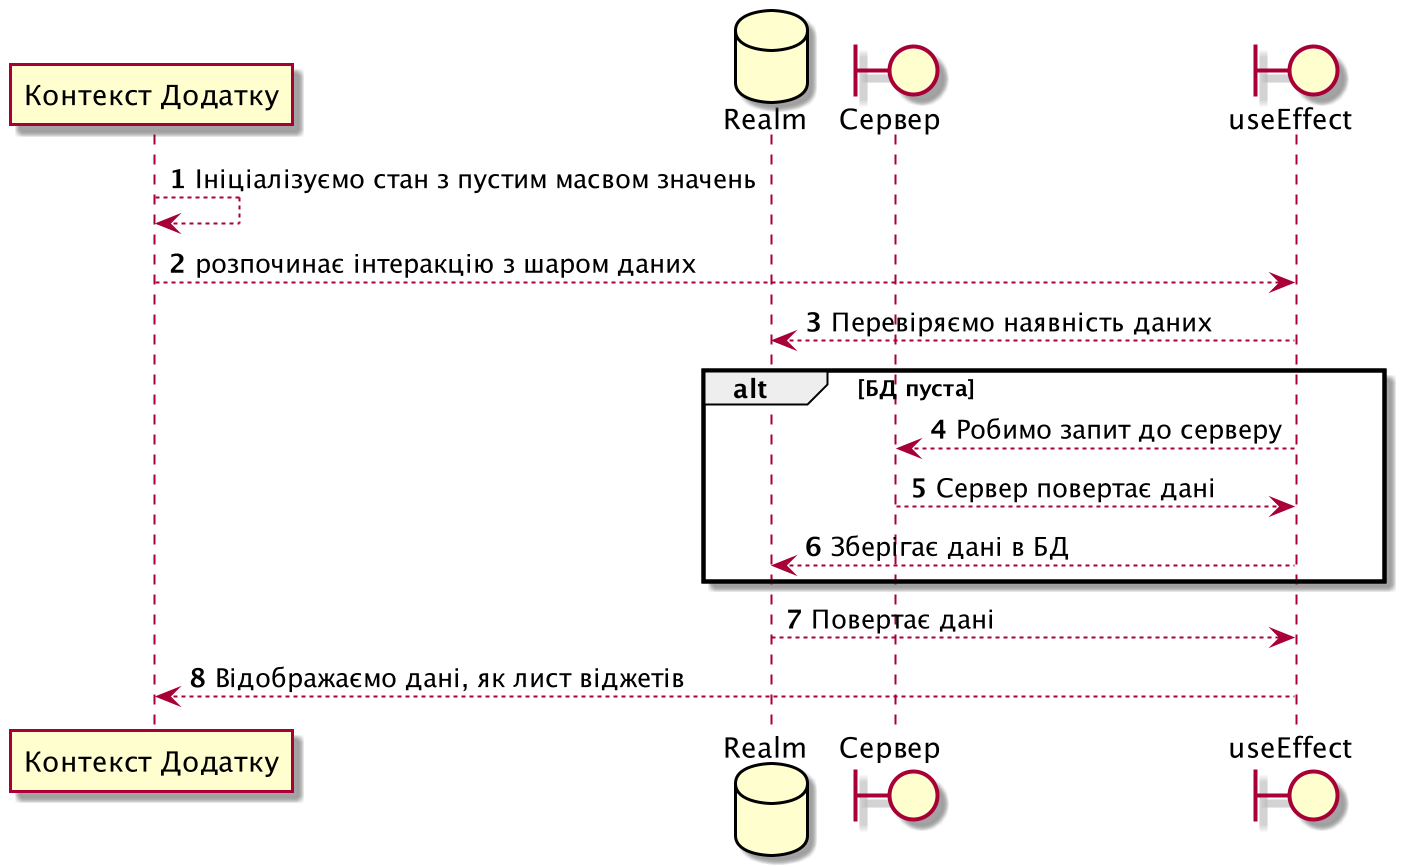
\includegraphics[scale=0.3]{app_widget.png}
        \caption{Схема послідовності віджету App та інтеракція з шаром даних}
        \label{fig:rn_realm}
    \end{center}
\end{figure}
